\documentclass{article}
\usepackage[utf8]{inputenc}
\usepackage{color}
\usepackage{mathtools}
\usepackage{graphicx}
\usepackage{hyperref}
\hypersetup{urlbordercolor={1 1 1}}


\begin{document}
The Structure of the thesis
\begin{enumerate}
    \item[1.] Motivation
        \begin{enumerate}
            \item[1.1] Python language overview
            \item[1.2] R language overview
            \item[1.3] Python vs R wars
            \item[1.4] Thesis description
            \item[1.5] Data preparation 
        \end{enumerate}
    \item[2.] Python
        \begin{enumerate}
            \item[2.1] The structure of the program
            \item[2.2] The process description
            \begin{enumerate}
                \item[2.2.1] Used Libraries
                \item[2.2.2] Documentation quality and quantity
                \item[2.2.3] Advantages and disadvantages of the program 
            \end{enumerate}
            \item[2.3] Results
        \end{enumerate}
    \item[3.] R
        \begin{enumerate}
            \item[3.1] The structure of the program
            \item[3.2] The process description
            \begin{enumerate}
                \item[3.2.1] Used Libraries
                \item[3.2.2] Documentation quality and quantity
                \item[3.2.3] Advantages and disadvantages of the program 
            \end{enumerate}
            \item[3.3] Results
        \end{enumerate}
    \item[4.] Results
        \begin{enumerate}
            \item[1.1] Objective comparison
            \item[1.2] Subjective comparison
            \item[1.3] Conclusion
        \end{enumerate}
    \item[5.] Literature
\end{enumerate}

\newpage
\section{Motivation}
Every time requires it's own heroes. Nowadays, with a massive digitalization of the world, statistical analysis is not only used in spheres like classical production and distribution (logistics), but also everywhere on the web. In order to create a nice web-site, that will attract buyers and more important will make them purchase things from a particular on-line shop using this exact site, on-line shops require an analysis of a customer's behavior, specific demands and preferences. Another example where data analysis is essential is video games industry. The AI, which is built in an immense data source and is constantly analyzing the incoming data from the players, servers and third party sources (if needed), is used in many game-projects from a simple browser-strategy to "the most expected game of the year". The game play, the enemies, the load distribution on the servers and many other things are based on analysis and forecast. The are many-many other examples where data analysis is used.\vspace{3mm}\\
Since the computer technologies are way more advanced, than they were several decades ago, the computations can be automatized, the data collection can be automatized. For every purposes certain tools, languages and libraries should be chosen carefully among the great choice. In this work we will concentrate our attention on a statistic-econometric task. On the whole, almost every language can be used to build a program for collecting, processing and visualizing data: SCALA, C, C++, .NET, Java, Python, JavaScript, R, etc.. However, some of the languages are more suitable for this purposes.\vspace{3mm}\\
In this work we will concentrate on "easy" languages. We will compare Python 3 (Python 2 in form of some libraries) language with R language. Both of them are relatively new (Python is about 25 years old and R is about 22 years old) to the wide publicity. Both are currently used for data analysis (for Python it is not the only use, but as we said before, we will concentrate on this aspect). Both languages are widely used in open source projects and have a large community behind them. Also, very important that both of the languages are relatively easy to begin with also for non-programmers. Python has a gradual learning curve due to its simplicity, clear and intuitive syntax. Although R has a steep learning curve it is still pretty easy to use for small and not too complex projects (which is the case for this thesis).

\newpage
\subsection{Python language overview}
The Python language is pretty young. It has first appeared about 25 years ago. As described on the official page in Wikipedia:"Python is a general-purpose, high-level programming language"[1]. That means that Python can be used for many tasks like back end development, front end development, data analysis and even for processor simulation (the python code will generate you VHDL code eventually). The language supports multiple programming paradigms: Object Oriented, Imperative and Functional programming.\\
Another big advantage of the language is being a cross-platform language executable via interpreter that can be installed on every operation system. Another possibility to run python programs without installing an interpreter is to package the program into stand-alone executable.\\ 
The language has an automatic garbage collector, so you don't have to worry about memory leaks by small to medium programs.\\
Enormous community stays behind Python and its \textcolor{blue}{variations}. The standard library has more than enough functions for easy start. The language's syntax is very clear and intuitive in comparison to C++, C or even Java. I would say the language is similar to normal human speech but in more strict and logical form.\\
Another good thing about Python is build-in test - doctest module. This test is very easy to use to check and debug your code on the fly. The use of the module is intuitively clear even to beginners. You also don't keep the test's text in other file, which gives you certain level of an overview of the program. Unit test are also widely used among the programmers using Python language. There also other possibilities to debug and benchmark the code written in python, but we will not discuss it here.\\
The disadvantage of the language is its speed in comparison with C, C++ and Java. Also the visualization tools could be better, but since the language is a multipurpose language, it is normal, that some things are not top among the class. \\

\subsection{R language overview}
According to Wikipedia:"R is a programming language and software environment for statistical computing and graphics"[5]. R is a successor of the S language, purposed about 39 years ago. R is distributed under GNU General Public license, which makes this language a nice choice for an open source analytical project.\\
Same as Python, R also uses interpreter to execute the code. R language is pretty much single-purpose language. The main use of R is statistical analysis and visualization. Since R is an open source project, there is a huge \textcolor{blue}{community of real life practice and scientists behind it}.\\
The disadvantage of the language is its one-purpose nature. Analytical project built with R will work with no doubt very fast and good, presenting good results. But the use of such project will be reduced, since there are very few quick and comfortable ways to integrate the program into the system.\\

\subsection{Python vs R wars}
Since both languages offer tons of packages and libraries for analyzing and visualization, people argue about what language is a better fit. You can find a lot of discussions about this topic on stackoverflow [6], stackoverflow analog for data science [7] and many other resources on internet [8],[9],[10].
So far nobody has managed to give a satisfactory final answer, since the languages indeed are different. However for every concrete task and scale we can give a list of requirements and compare the languages objectively leaving the subjective comparison aside.\\
Tho formal criteria to compare Python and R are:
\begin{enumerate}
    \item The amount of useful resources for the task
    \item Clear documentation with examples
    \item Performance
    \item Memory use
    \item Appropriate data structures
    \item Possibility to work with Big Data
    \item Visualization tools
    \item Hard or soft limitations
    \item Need of workarounds
\end{enumerate}
Using this list both languages can be objectively evaluated. These points are appropriate for all small-, middle- and big-projects. In next section we will describe the test-task to compare Python and R languages and define the points-system for objective evaluation.\\

\subsection{Thesis description}
The idea of this bachelor thesis is to test which language suits better specific statistic task. 
The program that will be evaluated consists of four parts:
\begin{enumerate}
    \item Getting and formatting data - the program should be able to read a prepared file in csv format. Afterwards, the program should format the data into needed structure for further use.
    \item Analyzing data - the program should be able to run statistical test to figure out data characteristics. This step is needed to determine what regression models are allowed for this data set. Following test will be presented: stationary test, build cdf and kde, find moments, distribution test (goodness of fit tests).
    \item Building a model - the program should be able to create a proper model using a step-forward algorithm, set the limits on the number of the predictors and return the names of the parameters, regression parameters and some useful statistics.
    \item Visualization - the program should be able to present the results and steps between if needed.
\end{enumerate}
The program will build a simple regression if possible. This task is considered to be middle-size task, not too easy but at the same time not too time and knowledge consuming.
The data will be prepared and provided as 2 files (training set and test set) in .csv format.\\
According to the list for objective evaluation, each point will give either 0 or 1 score to language. The 0 score will be given in negative case and score 1 will be given in positive case.
\begin{enumerate}
    \item[] Useful resources - at least 2 different libraries for one task gives 1 point.
    \item[] Documentation - examples, clean source code and clear structured APIs give 1 point.
    \item[] Performance - fastest language gets 1 point
    \item[] Memory - the program with the smallest memory use gets 1 point.
    \item[] Data structures - no additional formatting needed gives 1 point.
    \item[] Big Data - libraries, plugins and frameworks for big data give 1 point.
    \item[] Visualization - easiness in use and customization gives 1 point.
    \item[] Limitations - if there are any limitations, the language gets 0 points.
    \item[] Workarounds - additional time to solve the task gives 0 points (deviation from the time for the naive implementation).
\end{enumerate}
The results of the programs will be also compared. If they differ, the models will be cross-compared wit the other program or manually.\\
The task is to build a best matching linear regression (if possible) for a company (always the first column in the file) using certain limitations on the number of the predictors.

\subsection{Data preparation}
As was mentioned before the data set for this task will be prepared in advance. For our purpose we decided to take Intel as a dependent variable in the regression. Predictors will be chosen among the companies from the same market of micro controllers, supplier market and customers market.\\
The Intel's competitors can be found on Wikipedia listed in several tables for years from 1998 to 2013. We used a parser to get following list of manufacturers for the years 2000-2013 for semiconductors market:
\begin{verbatim}
['AMD', 'Qualcomm', 'Micron Technology','Hynix',
'Infineon Technologies', 'Intel Corporation', 
'STMicroelectronics', 'Texas Instruments']
\end{verbatim}
The semiconductors are the basic component for different devices, so the potential consumer-markets may vary. In this Bachelor we will concentrate on microchips (CPUs) consumers, following markets are: Tablets, Smart-phones, personal computers, automobiles, video game consoles, medical technologies, Engineering technologies, Aviation. Tablets and personal computers are united into one market-group.\\
Automobile market:
\begin{verbatim}
['Toyota', 'GM', 'Volkswagen', 'Ford', 'Nissan', 
'Fiat Chrysler Automobiles', 'Honda', 'PSA', 'BMW',
'Daimler AG', 'Mitsubishi', 'Tata', 'Fuji']
\end{verbatim}
The only significant players (manufacturers) on the game console market are: Microsoft, Sony and Nintendo.\\ 
The aviation market is presented by following companies: 
\begin{verbatim}
['Boeing', 'United Technologies', 'Lockheed Martin',
'Honeywell International', 'General Dynamics',
'BAE Systems', 'Northrop Grumman', 'Raytheon',
'Rolls Royce', 'Textron', 'Embraer', 'Spirit AeroSystems Holdings Inc.']
\end{verbatim}
The next market consuming microchips and other Intel-production is Smart-phones, Tablets and PCs. These gadgets are not substitutes, but they are all very similar in production-process, end-consumer and functions. Since many companies are presented on the markets mentioned above and have further production markets, we will put them into "Diversified" category. The diversified companies that may influence Intel are:
\begin{verbatim}
['Samsung', 'Apple', 'Microsoft', 'Nokia', 'Sony', 'LG',
'Motorola',  'Lenovo',  'BlackBerry', 'Alcatel', 'Vodafone']
\end{verbatim} 
Another huge consumer market for Intel is medical equipment market. The following companies present this sphere:
\begin{verbatim}
['Johnson & Johnson', 'General Electric Co.', 'Medtronic Inc.',
'Siemens AG', 'Baxter International Inc.', 
'Fresenius Medical Care AG & Co.', 'Koninklijke Philips',
'Cardinal Health Inc.', 'Novartis AG', 'Stryker Corp.',
'Becton, Dickinson and Co.', 'Boston Scientific Corp.',
'Allergan Inc.', 'St. Jude Medical Inc.', '3M Co.',
'Abbott Laboratories', 'Zimmer Holdings Inc.', 
'Smith & Nephew plc', 'Olympus Corp.', 'Bayer AG',
'CR Bard Inc.', 'Varian Medical Systems Inc.',
'DENTSPLY International Inc.', 'Hologic Inc.', 
'Danaher Corp.', 'Edwards Lifesciences', 'Intuitive Surgical Inc.']
\end{verbatim}
Additional to above mentioned companies several big players from the industrial equipment market will be added. These are following companies:
\begin{verbatim}
['ABB Robotics', 'Adept Technology', 'Bosch', 'Caterpillar',
'Denso Robotics', 'Google', 'Universal Electronics']
\end{verbatim}
The list of the potential predictors is not full, because some pretty big players on the markets are left due to the lack of information. The reason of the information-lack is recent enter to the international stock exchange (since 2010 earliest). Some companies are still closed for the foreign investors (which is the case for such giants as Samsung, Honda and other Asian companies). The last limit on chosen companies is the trading-volume. We simply can not use the company's data for composing a regression, if the last year or two the trade volumes for the shares was 0.\\
After the companies were chosen, the whole data table will be split into 2 data sets: learning set and validation set. We have obtained daily prices from 2006 to 2015 (31.12.2014 is the last date for all indexes). The training or learning set will be approximately 70\% from the whole data volume: from 2006 to 2010. The validation-set is about 30\%: from 2011 to 2012. For this work we use daily frequency (only opening prices).\\

\newpage
\section{Python}
\subsection{The structure of the program}
The program consists of three main classes, connected with each other in main class. The first class is called DataFormating.py and is responsible for getting data out of the csv file and writing it into an instance of a proper format for other two classes, also the dependent variable will be extracted from the whole data base (the dependent variable is always the first column in the csv table).\\
The second class is called StatisticTests.py, it runs several test to find out main static characteristics in order to choose an appropriate model class for the data.\\
The third class is called BuildModel.py. This class builds the multiple linear regression (according to the results of the StatisticTests class) using step-forward approach:
\begin{enumerate}
    \item The amount of companies taken into account is reduced using correlation: all companies with correlation less than 30\% are left out.
    \item A limit on the maximum number of the parameters is set using following rule: 1 company out of 10 if number of company exceeds 5.
    \item The first step is to find the best one parameter company using the highest correlation coefficient from the first step.
    \item All possible combinations for fixed company from the previous step and left companies are created. For all these combinations the linear regression using Generalized Least Squares approach [\url{https://en.wikipedia.org/wiki/Generalized_least_squares}].
    \item The best model among the class is chosen using AIC criterion.
    \item Best models among the classes are compared using likelihood ratio test. 
    \item If the bigger model is better and the limit of the predictors in regression is not achieved, the new small model is equal to old big model and repeat from step 4. The final result is the last big model.
    \item If the smaller model is better or/and the maximum number of parameters in the final regression is achieved, than the final result is either the small model or the last big model. 
\end{enumerate} 
At the end the full information for the best model is returned.

\subsection{The process description}
In this section the process of the coding is described: what difficulties and problems are encountered and how they were solved.
\subsubsection{Used Libraries}
In the course of writing the program several steps were implemented. As was mentioned above in the "Program structure" section, these steps are: extracting and preparing the data for further use, check statistic characteristics and build the model based on the results of the statistics. In order to build the program three main libraries were used:
\begin{enumerate}
    \item Base Python library[12].
    \item SciPy resource (unites six different libraries, in our case three were used explicitly)[13].
    \item Statmodels[14].
\end{enumerate}
The functions and data structures defined in the base library was used for every simple task, except simple mathematical computations, since there were faster implementations.\\
The second most used library in this work is NumPy,this library is the part of the SciPy source. NumPy offers many fast multi dimensional computations and assosiated multi dimensional structures. In our work we used this library to compute several statistic and build data for displaying graphs. As we mentioned before, the built-in library was not fast enough for our computation (for bigger data arrays numpy is almost not an arguable choice):
\begin{verbatim}
>>> x=[random.randint(0,10) for i in range(0,1500)]
>>> len(x)
1500

>>> mean_base = statistics.mean(x)
>>> mean_base
4.966
>>> cProfile.run('statistics.mean(x)')   
         4531 function calls in 0.006 seconds
        
>>> mean_numpy = numpy.average(x)
>>> mean_numpy
4.9660000000000002
>>> cProfile.run('numpy.average(x)')
         17 function calls in 0.001 seconds
\end{verbatim}   
As you can see, the NumPy implementation of the function "average" is more accurate and efficient (4531 intern calls vs 17 intern calls). The run time difference can be already shown on the list containing 1500 elements.\\
The third library with fundamental use is Pandas, this library is also a part of the SciPy source. This library provides high-performance data structures and associated functions for data analysis. This library can be used for generating, accessing and formatting data. In this work we used to get the data from our .csv file in a intuitive manner and to avoid unnecessary formatting steps. Also Pandas offers you a functionality to get the data directly from web sites like: Yahoo Finance, Google Finance, Google Analytics, etc.., although we didn't used it in our program. Fo example the method we used to read the data and returned it in Data.frame format, which can be easily sliced according to the needs of the program or formatted.
\begin{verbatim}
data = pd.read_csv(str(self.file_name))
cProfile.run('data = pd.read_csv("../data/LearningSet.csv")'
    3316 function calls (3238 primitive calls) in 0.024 seconds
\end{verbatim}
The LearningSet file is a table containing 78 companies with 1240 prices for each company, 477,6KiB.\\
The library used for drawing and saving graphs is very popular and for many other libraries is a default use. Matplotlib is also a part of the SciPy source. It offers you different types of graphs and formatting tools.
\begin{verbatim}
plt.title(3M)
plt.plot(bin_edges[1:], cdf)
plt.clf()
\end{verbatim}
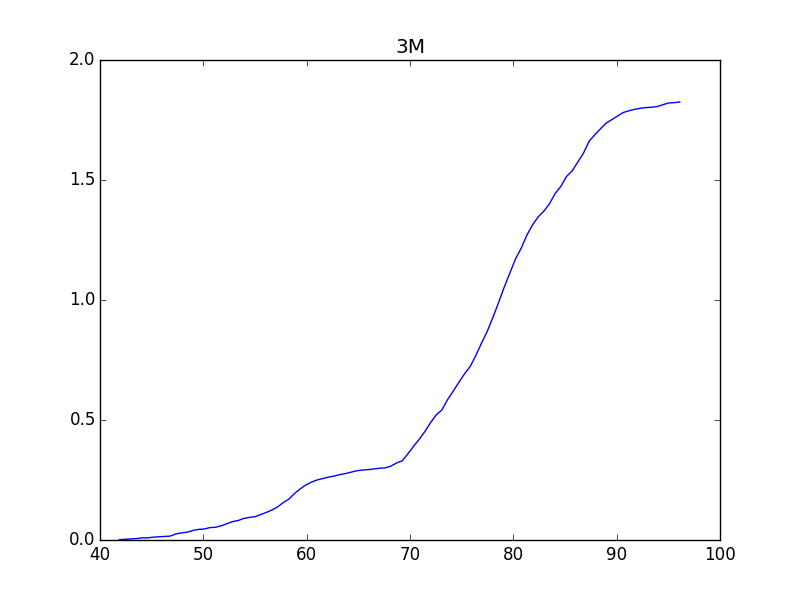
\includegraphics[scale=0.5]{PythonPlotExample.png} \\
The last but the fundamental library is Statmodels. This library offers a wide variety of tools and models for statistic purpose. Two main functions of the library used in our program are: Augmented Dickey-Fuller test for unit root and building a multiple linear regression with generalized least squares approach.
\begin{verbatim}
statistic = statmodel.adfuller(self.dict_data[key], 250, 
                        'ctt', 't-stat', False, False)[0] - stationary test
                        
model_null = sm.GLS(y, smaller_model_list)
info_small_model = model_null.fit().summary()
\end{verbatim}   

\subsubsection{Documentation quality and quantity}
The quality and the quantity of the documentation plays a crucial role for the project of every complexity, but especially for beginner levels. In this work we will evaluate the documentation of the languages and connected libraries, packages, frameworks using score system. The languages can get points for each position criterion given in the table:
\begin{enumerate}
    \item The documentation is always available.
    \item The documentation is easy to navigate.
    \item The documentation offers a sufficient amount of examples.
    \item The examples given in the documentation cover at least two complexity levels (a very simple use and use in an advance context).
    \item The documentation provide a link to the source code (mainly for non-base packages and libraries).
    \item For scientific libraries the theoretical background is provided.
    \item The documentation is easy to read (formatting, colors, description of the parameters and output).
\end{enumerate}
Originally, Python language was used a lot by the scientific society and many libraries were also implemented for scientific purpose by people with a certain background. In this work we have used base Python 3 library [12],  SciPy[14] and Statmodels[15]. SciPy unites several packages, only three from the whole list were used in our Python program: NumPy, Matplotlib and Pandas.\\
The Python program was written in Python 3 version, in this work we did not encountered any problems with the version conflicts. But it is possible that some external libraries are build on Python 2 and thus can cause some issues. In this case you can use Six library[16] to guarantee the compatibility of the versions. As we said, our program did not require use of this library, but it is safe to keep it in mind.\\
According to the provided evaluation table all four libraries will get points and the weighted (approximate weights are based on appearance frequency and importance of the library in the program) score will be added to the python total score.\\
The base Python library:
\begin{enumerate}
    \item 1 Point (the documentation was always available, no delays over period of 6 month were noticed).
    \item 1 Point (the web site is modern and have a very clear structure).
    \item 1 Point (each function has one simple example, some functions are explained by "identical function" example, at the end of the class description composite example is given).
    \item 1 Point (see above).
    \item 0 Point (the code is mostly not in a free access, mostly normal for base libraries).
    \item 1 Point (functions are either explained in the documentation, or provide a link to an external source, for example for math.gamma(x) the description link sends you to the Wikipedia page for gamma function).
    \item 1 Point (the Structure of the documentation for every class is the same and  mostly intuitive. You can navigate through the documentation using different methods: global index, glossary, etc.).
\end{enumerate}
From the SciPy source three libraries were used explicitly: NumPy, Matplotlib and Pandas. The documentation of the libraries contain more detailed information and some additional examples, but the structure and the formatting are the same according to python styling trend. So the SciPy documentation will be evaluated.
\begin{enumerate}
    \item 1 Point.
    \item 1 Point.
    \item 1 Point.
    \item 1 Point.
    \item 1 Point.
    \item 1 Point.
    \item 1 Point (similar styling pattern used for all libraries).
\end{enumerate}
The most important library for our python program was Statmodels, since we used it to build the models. Although the library itself is very powerful, it is not easy to use and to understand.
\begin{enumerate}
    \item 0 Point (the documentation is hosted on Sourceforge and the server was down for about a week during the program development).
    \item 0 Point (too many sub classes and sub methods, which importance you can not evaluate from the first view).
    \item 1 Point.
    \item 0 Point (basic examples are not always provided by the documentation).
    \item 1 Point (source code is hosted on github, thus no issues with availability, but very hard to read).
    \item 1 Point.
    \item 0 Point (the explanation order of the input parameters, output parameters and methods is alphabetical and not logical, the explanation is sometimes not sufficient).
\end{enumerate}
So the final score for the python documentation is:
\[ \frac{(\frac{2}{5}(6) + \frac{1}{5}(7) + \frac{2}{5}(3) )}{7}= 0.71\]


\subsubsection{Advantages and disadvantages of the program}
The end result is currently printed out to a console: the names of the companies in the final regression, main characteristics of the regression (AIC, BIC, Loglikelihood, coefficients and errors, etc.) and final run time of the program. 
The results of the program for the given data, described in the data preparation section are:
\begin{verbatim}
The best model contains  6  parameters. And the model is:
['STMElectro', 'Olympus', 'St Jude', 'Lenovo', 'MicronTech', 'Google']
                            GLS Regression Results                            
==============================================================================
Dep. Variable:                      y   R-squared:                       0.998
Model:                            GLS   Adj. R-squared:                  0.998
Method:                 Least Squares   F-statistic:                 8.701e+04
Date:                 Do, 24 Sep 2015   Prob (F-statistic):               0.00
Time:                        20:20:45   Log-Likelihood:                -1753.3
No. Observations:                1239   AIC:                             3519.
Df Residuals:                    1233   BIC:                             3549.
Df Model:                           6                                         
Covariance Type:            nonrobust                                         
==============================================================================
                 coef    std err          t      P>|t|      [95.0% Conf. Int.]
------------------------------------------------------------------------------
x1             0.1254      0.016      7.933      0.000         0.094     0.156
x2             0.0609      0.012      5.065      0.000         0.037     0.085
x3             0.3261      0.016     21.029      0.000         0.296     0.357
x4             0.2126      0.004     47.272      0.000         0.204     0.221
x5             0.0083      0.001     12.929      0.000         0.007     0.010
x6             0.1291      0.012     10.536      0.000         0.105     0.153
==============================================================================
Omnibus:                       10.831   Durbin-Watson:                   0.120
Prob(Omnibus):                  0.004   Jarque-Bera (JB):               10.859
Skew:                           0.212   Prob(JB):                      0.00439
Kurtosis:                       2.827   Cond. No.                         357.
==============================================================================

[Finished in 13590.5s]
\end{verbatim}
As you can see, the first and biggest disadvantage is the run time. The program runs for 3,7 hours.\\
 The main time consumption comes from StatisticTests.py, specifically from stationarity test. \textcolor{red}{verbatim - run time}Since the naive implementation was used for writing the test section, the main time consumption is also presented in this part of the program. The advantage of the python is its multipurpose nature. It is possible to speed up all functions that change arrays or other data structures using speed up methods like Multiprocessing [21]. This will give you up to 8 times speed up momentum (depending on number of cores you can use). However this a bit of intermediate knowledge of python programming and will be quite difficult for a beginner to use.\\
Another disadvantage of the program written in python is the time you have to invest into the language investigation, since there are concepts and non-intuitive implementations. For instance:
\begin{verbatim}
>>> a = {"a":[1,2,3], "b":[1,2,3], "c":[1,4,9]}
>>> b = a
>>> b["a"] = [1,4,9]
>>> b
{'b': [1, 2, 3], 'a': [1, 4, 9], 'c': [1, 4, 9]}
>>> a
{'b': [1, 2, 3], 'a': [1, 4, 9], 'c': [1, 4, 9]}
\end{verbatim} 
Although we haven't expected dictionary a to change. Python does not implicitly copies objects. The example above shows how two objects are referred to the same object. Thus during mutating one of the objects, all references will change in order to keep referring to the object in its current state. This can be crucial for the program, since we have used one originally formatted dictionary for different purposes. In order to avoid this error you need to do following thing:     
\begin{verbatim}
>>> a = {"a":[1,2,3], "b":[1,2,3], "c":[1,4,9]}
>>> b = a.copy()
>>> a
{'b': [1, 2, 3], 'a': [1, 2, 3], 'c': [1, 4, 9]}
>>> b
{'c': [1, 4, 9], 'b': [1, 2, 3], 'a': [1, 2, 3]}
>>> b["a"] = [0]
>>> b
{'c': [1, 4, 9], 'b': [1, 2, 3], 'a': [0]}
>>> a
{'b': [1, 2, 3], 'a': [1, 2, 3], 'c': [1, 4, 9]}
\end{verbatim}
or 
\begin{verbatim}
>>> a = {"a":[1,2,3], "b":[1,2,3], "c":[1,4,9]}
>>> b = dict(a)
>>> b
{'c': [1, 4, 9], 'b': [1, 2, 3], 'a': [1, 2, 3]}
>>> b["a"]=[0]
>>> b
{'c': [1, 4, 9], 'b': [1, 2, 3], 'a': [0]}
>>> a
{'b': [1, 2, 3], 'a': [1, 2, 3], 'c': [1, 4, 9]}
\end{verbatim}
Such thing can confuse not only very beginners, but also advanced programmers, because you need to keep every thing in mind.\\
The first really big advantage of the python language is testing. Python has built-in doc-tests [22], that are incredibly easy to use. We will not discuss this theme in details, since the tutorials and the documentation are very easy. Another test possibility are Unit Tests [23]. Python language gives the programmer many ways to test and debug the program in order to avoid possible computational and logic errors.\\
The second advantage of the program in python is actually beyond the scope of this work. Working with the whole process (data mining, data processing and data visualization) in real time and with feedback if needed can't be implemented in R. So, if you are writing an interactive application, than you should definitely go for python.

\subsection{Results}
To sum up the objective arguments of using python for writing a small program to compute a linear regression for a given data and restrictions, we will sum up the points from the table from the thesis description section.
The points for the Python program are:
\begin{enumerate}
    \item Useful sources: 1 Point.
    \item Documentation: 1 Point (arguable for some libraries, but in general the documentation is on a high level).
    \item Performance: 0 Points.
    \item Memory: 0 Points (Since the data format for different packages is different, our program have used a combination of different data structures to store all formats).
    \item Data structures: 0 Points (different libraries uses different shapes).
    \item Big Data: 1 Point (Python have tools for Big Data analysis, or can be used with known tools like Hadoop, Cassandra, Pig, Hive, etc.).
    \item Visualization: 1 Point (several libraries also for displaying the chart in web).
    \item Limitations: 1 Point (accept time to actually learn the language there are no limitations).
    \item Workarounds: 1 Point (for this particular task there have always been a method or several wrap functions).
\end{enumerate} 
The Python program gets 6 points in total.

\newpage
\section{R}
\subsection{The structure of the program}
The program written in R language has the same structure as the Python program. The R program consists of three classes: DataFormatting.r, StatisticTests.r and BiuldModel.r. Their functions are similar to the same functions from the first program. However there are slight differences in the inner functions of the classes.\\
The R language is very convenient in terms of data formatting - you don't need it. The object called Data.frame is returned when using read.csv() from the base package. This object has methods that allow the programmer to use the data directly without extracting it and saving to the proper format. For example the list of all companies from the table was extracted using the function "colnames(data.frame)" as an output we get the list object containing the elements from the first row of the table. So the R program does not have inner helpers - converter functions.\\
The The StatisticTests.r runs tests to detect statistic characteristics of the data: Kolmogorov-Smirnov goodness of fit distribution test, Augmented Dickey-Fuller test to detect unit root, build cumulative distribution function and kernel density function, find main characteristics (mean, standard deviation, skew, kurtosis).\\
The third class creates the model following the same steps from the step-forward approach that was used in the Python program:
\begin{enumerate}
    \item Cut off all companies with correlation less than 30\%.
    \item Set the limit for the maximum number of parameters in the final regression. 
    \item Choose the best one parameter model.
    \item Build all possible tuple-combinations with fixed parameter.
    \item Choose the best model among the two parameter class.
    \item Compare the best models from two different classes via Likelihood Ratio Test.
    \item Repeat until the smaller will be better or/and the maximum number of parameters is reached.
\end{enumerate}
\subsection{The process description}
In this section the process of the program writing is described in more details: what packages were used, what difficulties appeared, etc..
\subsubsection{Used Libraries}
For this R program following packages were used:
\begin{enumerate}
    \item Base package[16].
    \item Stats package[17].
    \item Nlme package[18].
    \item Tseries package[19].
\end{enumerate}
The first base library was used for all basic computations like moments, correlation vector, etc.. This package provides many different functions for formatting the data. For example:
\begin{verbatim}
formula <- as.formula(paste(dep$name,"~", as.character(names(small_model)), collapse=""))
\end{verbatim}
This function converts the string object from the brackets into a formula object that is further used as an input parameter for building a linear regression using GLS method. The base package offers basic math operation as well.\\
The StatisticTests.r class uses both stats and tseries packages to build statistic tests on the data. The tseries package offers many different tests and methods used in computational finances and time series analysis. In this work we have only used Agumented Dickey-Fuller test to test the data for stationarity:
\begin{verbatim}
test <- adf.test(data[[company]])
\end{verbatim}
The second package used in StatisticTests class offers functions to run simple statistic tests on the data and build simple characteristics. In our work we have used the stats package to build graphs for each company from the data table and test the data for its distribution. The program has yields the same results as the python program.\\
The fourth package used in this program offers the the possibility to build linear regression using given parameters. The use of the functions from the library are very intuitive:
\begin{verbatim}
small <- gls(as.formula(paste(dep$name,"~", as.character(names(small_model)), collapse="")), data)
\end{verbatim} 
Where the first parameter is from the class formula looks like string object: "Intel ~ Olympus + St.Jude". The second parameter is the data, where the variables from the formula match the names of the columns from the data frame object.\\
The program is run from the console from the R environment. The result is also printed out to the console. The result contains log-likelihood of the final regression, its companies, coefficients, AIC and BIC. Additional information provided by the nlme package offers the correlation matrix for given parameters.  
\subsubsection{Documentation quality and quantity}
In comparison to the Python language, R was build only for analytical purpose. The most part of the contributors are scientific institutions, and thus the R language documentation is written in a scientific paper style. \\
Although the functions offered by the chosen libraries have covered all the need of the program written in this work, there were difficulties to understand how the function should be used, especially since R language requires a certain time investment to get started.
\subsubsection{Advantages and disadvantages of the program}
\subsection{Results}

\newpage
\section{Results}
\subsection{Objective comparison}
\subsection{Subjective comparison}
\subsection{Conclusion}

\newpage
\section{Literature}
\begin{enumerate}
    \item \url{https://en.wikipedia.org/wiki/Python_(programming_language)}
    \item
    \item \url{https://www.r-project.org/about.html}
    \item \url{http://www.revolutionanalytics.com/what-r}
    \item \url{https://en.wikipedia.org/wiki/R_(programming_language)}
    \item \url{http://stackoverflow.com/questions/2770030/r-or-python-for-file-manipulation}
    \item \url{http://datascience.stackexchange.com/questions/326/python-vs-r-for-machine-learning}
    \item \url{http://www.kdnuggets.com/2015/05/r-vs-python-data-science.html}
    \item \url{http://blog.datacamp.com/r-or-python-for-data-analysis/}
    \item \url{http://101.datascience.community/2015/05/12/data-science-wars-r-vs-python/}
    \item
    \item Python 3 \url{https://www.python.org/doc/}
    \item SciPy \url{http://www.scipy.org/}
    \item Statmodels \url{http://statsmodels.sourceforge.net/}
    \item Six \url{https://pythonhosted.org/six/}
    \item Base R library \url{https://stat.ethz.ch/R-manual/R-devel/library/base/html/00Index.html}
    \item Stats R library \url{https://stat.ethz.ch/R-manual/R-patched/library/stats/html/00Index.html}
    \item Nlme R library \url{https://cran.r-project.org/web/packages/nlme/nlme.pdf}
    \item Tseries R library \url{https://cran.r-project.org/web/packages/tseries/tseries.pdf}
    \item \url{}
    \item \url{}
\end{enumerate}
\end{document}